\section{Publicization of academic software}
\label{study1}

The \textit{publicization of academic software} is concerned with making
the software explicitly available from a given URL cited or written down in a software
publication (a scientific paper published by its authors). 
Essential features from academic software after its publicization include the format in
which they are made available (binary or source code), the types of licenses
used, and other issues related to their distribution.

\myparagraph{Scoping}
%
The goal of the study is to
analyze the {\it static analysis software projects published as academic software}
with the purpose of \textit{characterizing their publicization}
concerning the \textit{url, license, source code, and download availability} in
the perspective of \textit{scientists end-users} in the context of
\textit{software publications of ASE and SCAM conferences}.


In this context, we investigated four research questions:

\newcommand{\StudyOneQuestionOne}{
	\textbf{(RQ1.1)} \textit{Does academic software for static analysis published in ASE and SCAM
papers have an official online presence?}
}
\newcommand{\StudyOneQuestionTwo}{
	\textbf{(RQ1.2)} \textit{Is academic software for static analysis published in ASE and SCAM
papers available for download?}
}
\newcommand{\StudyOneQuestionThree}{
	\textbf{(RQ1.3)} \textit{Is the source code of academic software for static analysis published
in ASE and SCAM papers available?}
}	
\newcommand{\StudyOneQuestionFour}{
	\textbf{(RQ1.4)} \textit{Does academic software for static analysis published in ASE and SCAM
papers with source code available provide a free software license?}
}

\noindent \StudyOneQuestionOne By ``official online presence'' we mean
that there is an official website or project repository; an URL with
information from the software, usually maintained by the authors of the
software themselves.

\noindent \StudyOneQuestionTwo We investigated if it is possible to
download the software so that independent authors can use and
evaluate the software, or for reproducibility of studies using the software, or
for further research purposes with software support.

\noindent \StudyOneQuestionThree We analyzed if researchers and other
actors interested in details about the construction of the software and present
in the source code itself will have access to this knowledge, which is usually
part of the research itself. The access to the source code is also useful for
those who have an interest in the use, eventual adaptations or fixes that may
be required to run in other environments or operating systems.

\noindent \StudyOneQuestionFour We verified if the projects have
explicit permission for contributions to the source code in a way that can be
adapted to meet emerging needs and that these adaptations can also be
distributed freely.

Measurements required in this study include:
(1) the number of projects with a given name and URL;
(2) the number of projects with available URL;
(3) the number of projects available for download;
(4) the number of projects with source code available; and
(5) the number of projects that use free software licenses.

\myparagraph{Data Collection}
%
The literature review found 61 software publications
on academic software for static analysis
among the 1873 papers published at the ASE between 1991 and 2015 and SCAM between 2001 and 2015.
Figure~\ref{papers-and-tool-papers-selected-by-year}
presents the number of software publications by year
comparing them to the total number of publications.

\begin{figure}[ht]
  \center
  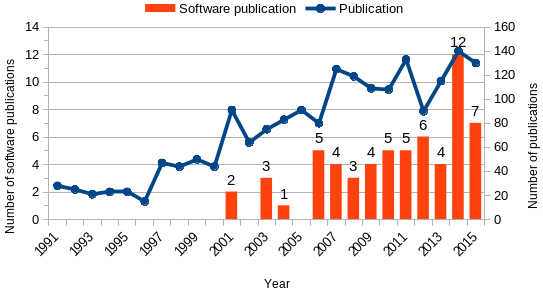
\includegraphics[scale=0.6]{figs/papers-and-tool-papers-selected-by-year-2axis.png}
  \caption{Number of selected software publications.}
  \label{papers-and-tool-papers-selected-by-year}
\end{figure}


\begin{table}[ht]
\scalefont{0.9}
\caption{Inclusion criterion and keywords}
\centering
\begin{tabular}{ p{4cm} l }
  \hline
  {\bf Criteria}                           & {\bf Keywords}                        \\
  \hline
  Mentions the project, software or tool   & {\tt tool} or {\tt framework}         \\
  Makes software available for download    & {\tt download} or {\tt available}     \\
  Identifies project URL                   & {\tt http}, {\tt https} or {\tt ftp}  \\
  Static analysis domain                   & {\tt static analysis} or {\tt parser} \\
  \hline
\end{tabular}
\label{screening-criterias}
\scalefont{1}
\end{table}


\begin{table}[ht]
\scalefont{0.9}
\caption{Inclusion criterion for extraction \cite{howison2016software}}
\centering
\begin{tabular}{ l p{6cm} }
  \hline
  {\bf Criteria}   & {\bf Explanation} \\
  \hline
  Identifiable     & Is it possible to identify a software project among the outputs of the article? (e.g., ``a program we wrote'', ``our implementation'', ``our prototype'' etc) \\
  Available        & Can we find mention to the URL for download the software project? \\
  \hline
\end{tabular}
\label{extraction-criterias}
\scalefont{1}
\end{table}

We followed semi-automated steps to carried the data collection. First, we
downloaded all PDF papers manually from both conferences, and then we applied
an automated filter\footnote{\url{https://github.com/joenio/dissertacao-ufba-2016/blob/master/bin/filter-papers}}
to perform a full-text search inside each file looking for the terms described
in Table \ref{screening-criterias}.
%
Finally, we inspected manually all filtered papers matching the criteria in
Table \ref{screening-criterias}, following the criteria presented in Table
\ref{extraction-criterias}. In short, we found a total of \SoftwareCount \
academic software projects among the 61 software publications, as listed at the
repository of this work\footnote{The list of all \SoftwareCount \ projects is available at \url{https://github.com/joenio/dissertacao-ufba-2016/releases/download/2018-03-26/apendices.pdf}}.


\myparagraph{Results and Analysis}
%
We have following implications:

\paragraph{\bf Official online presence}
Regarding question \textbf{RQ1.1}, from \SoftwareCount \ academic software
for static analysis, \SoftwareUrlNotAvailableCount \ do not have an official
online presence at the URL informed by their authors, and
\SoftwareUrlAvailableCount \ projects are available from the provided URL, that
is, the URL was found and is active.

\begin{figure}[ht]
  \center
  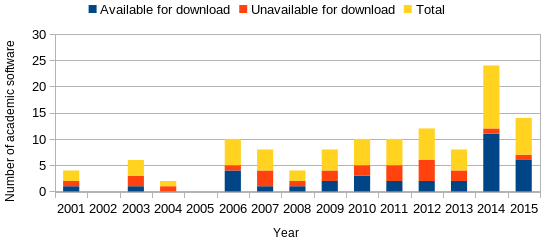
\includegraphics[scale=0.6]{figs/software-available-by-year.png}
  \caption{Number of projects available for download.}
  \label{software-available-by-year}
\end{figure}

\paragraph{\bf Sofware available for download}
About \textbf{RQ1.2}, from  \SoftwareCount \ selected projects,
with respect to the remaining \SoftwareUrlAvailableCount \ projects
that have online presence through the URL informed in the paper,
\SoftwareDownloadNotAvailableCount \ projects (40\%) are not available for
download.
This means that the authors informed an URL in
their paper, where software should be available,
but the URL is no longer available,
and the academic software cannot be found.
%
The remaining \SoftwareDownloadAvailableCount \ projects (60\%) are
available for download. Figure \ref{software-available-by-year} presents a summary of the
number of projects available for download per year.

\paragraph{\bf Source code available}
About \textbf{RQ1.3},
from \SoftwareDownloadAvailableCount \
academic software projects available for download,  only 2 -- FaultBuster
and Loopfrog -- did not make the source code
public. Both can be downloaded at no cost, in binary code. The remaining 34
projects are their source code available.

\paragraph{\bf Software license available}
Regarding \textbf{RQ1.4},
from \SoftwareCount \ academic software projects
(34 projects with the source code available),
13 did not provide any software license,
and 21 used free software license such as:
Affero General Public License,
Apache License,
BSD License,
Eclipse Public License,
FrontEndART Software Ltd,
GNU General Public License,
GNU Lesser General Public License,
Illinois/NCSA Open Source License, and
SAnToS Lab Open Academic License.
%
This means that only 21 projects (35\%) can receive contributions openly;
the remaining 13 projects (21\%) can receive contributions,
but improvements or fixes cannot be redistributed without prior authorization of
the authors.

\myparagraph{Threats to validity}
%
Automatic screening may have excluded from the review process existing software
publications on source code analysis. Selected software publications come from
a specific domain,  and only two software engineering conferences so that
results may have a linked bias to this domain and these two events.
Availability of downloadable software using only the URL informed by its
authors can lead to false negatives since this URL can change over time. This
threat, although not addressed, does not invalidate our conclusions,  since the
study aimed to evaluate the URL indicated by the original authors as well.
